% ===== 第 1 章 江口徹“ミラー対称性とは” PDF 10-25 / 原书 p.2-17 =====
\chapter{什么是镜像对称}
\chaptersub{Calabi--Yau 流形与超弦理论}
\chapterauthor{江口徹}{[京都大学基礎物理学研究所]}

% ===== PDF p.010 (原书 p.2) =====
mirror symmetry（镜像对称）这个说法，很多读者大概都听说过吧？它是在超弦理论的发展过程中
被发现的一个重要几何发现。近 15 年来，它一直是现代数学的重要研究主题，相关研究相当活跃。
超弦理论、规范理论、共形场论等数理物理所触发的数学研究，已经产生了许多重要结果；
而在这些研究之中，可以说镜像对称带来的冲击最大。

为说明镜像对称，我们先从超弦理论的紧化谈起。在超弦理论中，人们认为所有基本粒子
都对应着极短的“弦”（长度约 $10^{-33}$ cm）的各种运动状态。弦有两大类：
\textbf{闭弦}（closed string）与\textbf{开弦}（open string）。把闭弦量子化，其最低能量（基态）
中会出现自旋为 2、质量为零的状态；把开弦量子化，最低能量处则出现自旋为 1、质量为零的状态。
自旋 2、质量零的状态被看作\textbf{引力子}（量子化引力场时出现的粒子），
自旋 1、质量零的状态被看作\textbf{规范粒子}（量子化规范理论时出现的粒子）。
因此，只要忽略激发态、只看低能现象，闭弦就再现通常的引力理论（爱因斯坦的广义相对论），
开弦则再现规范理论的结果（参看图 1）。弦拥有的无数激发态，在宇宙早期那样的超高能
（极微观）世界里扮演重要角色，起着修正广义相对论与规范理论的作用。

广义相对论在微观世界会遇到困难，这一点早为人知。若把通常的量子化程序套用到广义相对论上，所有的计算都会给出量为无穷大的无意义结果。构造量子引力理论，曾是 21 世纪理论物理学留下的最大课题之一。

% ===== PDF p.011 (原书 p.3) =====
\begin{figure}[t]
  \centering
  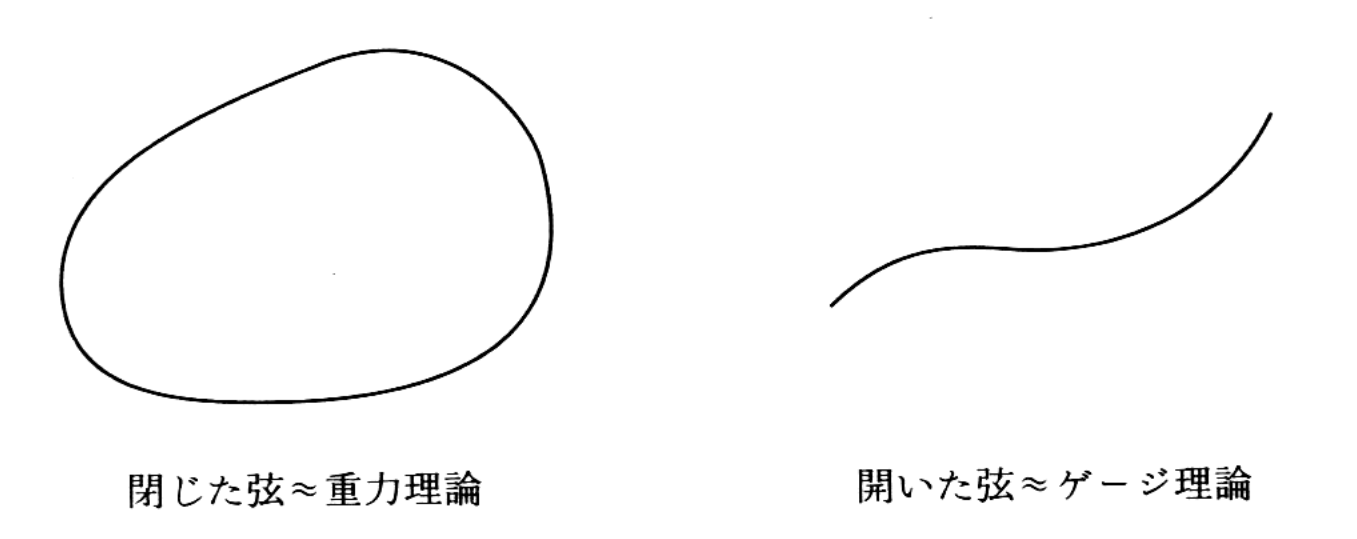
\includegraphics[width=0.86\linewidth]{figures/ch01-fig1.png}
  \figtitle{1}{闭弦 $\approx$ 引力理论，开弦 $\approx$ 规范理论（原书 p.3）}
\end{figure}

超弦理论正是这样一种量子引力理论：它克服了广义相对论在上述微观尺度上的困难。
人们相信，借助超弦理论，我们就能依据物理定律来讨论宇宙创生时全部物质聚集于一点的过程，
也能讨论巨大物质坍缩所形成的黑洞奇点。因此，如今超弦理论作为基本粒子的统一理论，被寄予了厚望。

话说回来，各位也许已经听说过：超弦理论只能自洽地存在于 10 维空间之中。
之所以选中 10 维，是因为理论的共形不变性，这一点无法更改。现在设弦延伸方向的参数为
$0\le \sigma\le 2\pi$，与时间对应的参数为 $\tau$，则弦在 10 维空间中的坐标可写作
\begin{equation}
  X^{\mu}(\tau,\sigma),\qquad \mu=0,1,2,\dots,9 \tag{1}
\end{equation}
弦一运动，其轨迹就在 10 维时空 $M^{9,1}$ 中张成一张曲面。可以把它看成由 $\sigma,\tau$
两个参数张出的区域，即\textbf{世界面} $\Sigma$，到 10 维空间的像（参看图 2）。
定义复数 $z=e^{\tau+i\sigma}$，世界面就成为（带有复结构的）黎曼面。
没有边界的黎曼面对应闭弦的运动，有边界的黎曼面对应开弦。
参数 $\sigma,\tau$ 的取法有任意性，因此要描述弦本身固有的力学，就必须让理论不依赖于参数的选法。
弦理论的\textbf{共形不变性}（conformal invariance）正是用来消去这种对参数取法的依赖性的，
它是弦理论的根基性对称性。

% ===== PDF p.012 (原书 p.4) =====
\begin{figure}[t]
  \centering
  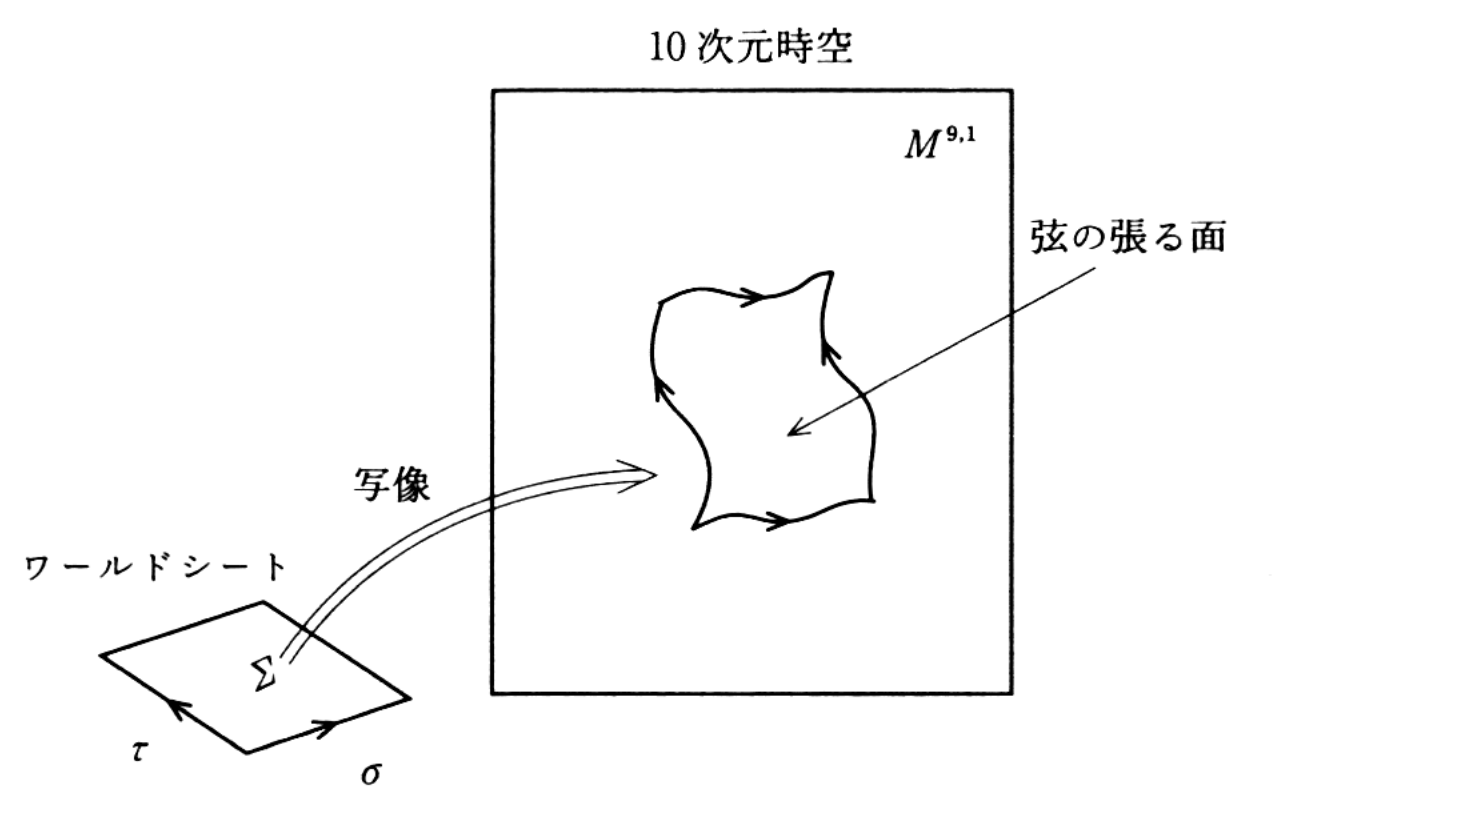
\includegraphics[width=0.9\linewidth]{figures/ch01-fig2.png}
  \figtitle{2}{世界面 $\Sigma$ 在 10 维时空 $M^{9,1}$ 中的像（原书 p.4）}
\end{figure}

共形变换定义为 $z\to f(z)$，其中 $f(z)$ 是 $z$ 的任意全纯函数。也就是说，
把世界面的坐标 $z$ 任意换成 $f(z)$，理论仍须保持不变（或共变）。
具有这种性质的二维场论，一般称为\textbf{共形场论}，它有着独特而优美的性质。

接下来考虑 10 维时空具有 4 维闵可夫斯基空间 $M^{3,1}$ 与 6 维（内部）空间 $K$ 之积
$M^{3,1}\times K$ 的形状的情形。这时，为使理论的共形不变性得以保持，允许的空间 $K$
会受到特别的限制。进一步要求 $M^{3,1}$ 上的理论具有超对称性，内部空间 $K$ 就必须是一种
称为 \textbf{Calabi--Yau 流形}的特殊流形。内部空间 $K$ 的尺度很小（约 $10^{-33}$ cm，
与弦长相当），日常生活中看不到它的延展，于是时空看上去就是 4 维的。
这样的设定称为弦理论的 \textbf{Calabi--Yau 紧化}（compactification）。

Calabi--Yau 流形是复维数为 3 的 Kähler 流形，但具有一种特殊性质：曲率的一部分，
即 $U(1)$ 部分为零。在 Kähler 流形上，曲率的 $U(1)$ 部分对应 Ricci 张量，
因此 Calabi--Yau 条件归结为\textbf{Ricci 平坦条件}
\begin{equation}
  R_{IJ}(g)=0,\qquad I,J=1,2,\dots,6 \tag{2}
\end{equation}
其中 $R_{IJ}$ 是 Ricci 张量，$g$ 是度量。

% ===== PDF p.013 (原书 p.5) =====
弯曲空间中的弦理论在经典层面具有共形不变性，但量子化之后一般会失去共形不变性。
此时，破坏共形不变的量子效应正比于 Ricci 张量。而在 Calabi--Yau 流形上 Ricci 张量恰好为零，
因此可以保证弦理论在量子化之后仍然保持共形不变性。

下面讨论 Calabi--Yau 流形 $K$ 的形变自由度，即\textbf{模空间}。现在把流形的度量 $g$
稍作改变，记为 $g+\delta g$。若要求新度量也满足 Ricci 张量为零，就得到
\begin{equation}
  R_{IJ}(g+\delta g)=0 \tag{3}
\end{equation}
此时 $\delta g$ 表示 Calabi--Yau 流形的模。把（3）关于 $\delta g$ 展开到一阶，得
\begin{equation}
  \Delta_{L}(g)\,\delta g=0 \tag{4}
\end{equation}
这里 $\Delta_{L}(g)$ 称为 \textbf{Lichnerowicz 拉普拉斯算子}，$\delta g$ 相当于该算子的
零特征值的特征函数。

用复坐标 $i=1,2,3$、$\bar j=\bar1,\bar2,\bar3$ 来表示，（4）的解可以分成两类：$g$ 的
(1,1) 型扰动 $\delta g_{i\bar j}$，以及 (2,0) 型或 (0,2) 型的 $\delta g_{ij}$
（或 $\delta g_{\bar i\bar j}$）。由于原来的 Kähler 度量 $g$ 是 (1,1) 型，(1,1) 型解仍保持 (1,1) 型，
这样的形变称为 \textbf{Kähler 形变}。另一方面，(2,0)（或 (0,2)）型解会与
(1,1) 型的 $g$ 相混，这意味着全纯坐标与反全纯坐标的定义发生了改变；因此这类自由度称为
\textbf{复结构形变}。

已知 Calabi--Yau 流形上 Kähler 形变的个数为 $h_{1,1}(K)$，复结构形变的个数为 $h_{2,1}(K)$。
这里 $h_{p,q}(K)$ 称为 \textbf{Hodge 数}，表示流形 $K$ 上 $(p,q)$ 型调和微分形式的个数
（$h_{p,q}=h_{q,p}$）。

最典型的 Calabi--Yau 流形之一，是 4 维复射影空间 $\PP^4$ 中的五次超曲面
（quintic）：
\begin{equation}
  \begin{aligned}
    & z_1^5+z_2^5+z_3^5+z_4^5+z_5^5-5\psi z_1z_2z_3z_4z_5=0,\\
    & (z_1,z_2,z_3,z_4,z_5)\in \PP^4
  \end{aligned} \tag{5}
\end{equation}
其中 $\{z_i\}$ 是 $\PP^4$ 的齐次坐标，$\psi$ 是复结构形变的参数之一。
对五次 Calabi--Yau 流形，有
\begin{equation}
  h_{2,1}=101,\qquad h_{1,1}=1 \tag{6}
\end{equation}

% ===== PDF p.014 (原书 p.6) =====
由（6）可知，五次超曲面有一百多个复结构形变模。一般地，Calabi--Yau 流形拥有
100--200 个量级的形变自由度。

所谓 Calabi--Yau 流形的\textbf{镜像对称}，首先是这样一种主张：给定一个 Calabi--Yau 流形
$K$ 及其 Hodge 数 $h_{1,1}(K),h_{2,1}(K)$，存在另一个 Calabi--Yau 流形 $\tilde K$，
其 Hodge 数为
\begin{equation}
  h_{1,1}(\tilde K)=h_{2,1}(K),\qquad h_{2,1}(\tilde K)=h_{1,1}(K) \tag{7}
\end{equation}
流形 $\tilde K$ 被认为与 $K$ 处于某种镜像关系，因此也称为 $K$ 的\textbf{镜像}。
如后文所见，借助这层镜像关系，人们可以用 $\tilde K$ 的周期积分理论来数 $K$ 中
所含全纯曲线的条数等等，\textbf{计数几何}（enumerative geometry）由此取得了显著进展。
此外，把复几何与辛几何联系起来的深刻数学研究也在推进。

\section*{N=2 共形场论}
\addcontentsline{toc}{section}{N=2 共形场论}

在进入这些话题之前，先介绍镜像对称的发现经过。如前节所述，
弦理论中共形变换下的不变性（或共变性）起着重要作用，因此可以把它看作一种共形场论。
对超弦理论而言，则是带超对称性的\textbf{超共形场论}。\textbf{超对称性}（supersymmetry）
如今被视为基本粒子论最基本的对称性之一。当自旋相差 $1/2$ 的玻色子（自旋为 $0,1$ 等整数的粒子）
与费米子（自旋为 $1/2,3/2$ 等半整数的粒子）总是成对存在时，理论就具有这种对称性。
超对称理论由于玻色子与费米子的自由度保持良好平衡而具有许多好性质：真空能量严格为零、
存在各种非重整化定理等显著结果都是已知的。

一般地，在只有玻色子的理论中加入费米子，可以把它变成具有超对称性的理论；
但让它带几重超对称性是有自由度的。对二维共形场论，可以赋予 $N=1,2,4$ 重超对称性；
而紧化在 Calabi--Yau 流形上的弦理论，已知可以由 $N=2$ 的超共形场论来描述
% ===== PDF p.015 (原书 p.7) =====
（这源于 Calabi--Yau 流形上 Ricci 张量为零、$U(1)$ 部分的不变性得以保留。）

共形场论的一般特征在于：理论中出现的场 $\Phi(z,\bar z)$ 可以分解为只依赖 $z$
与只依赖 $\bar z$ 的两个部分。
\begin{equation}
  \Phi(z,\bar z)=\phi(z)\bar\phi(\bar z) \tag{8}
\end{equation}
因此，$N=2$ 超共形变换也分解为作用于全纯场的分量（左手分量）与作用于反全纯场的分量（右手分量）。
下面先讨论左手分量。

二维共形变换本来是用任意解析函数 $f(z)$ 定义为 $z\to f(z)$ 的，因此构成一个具有无穷多个
生成元的无穷维李代数。先看无穷小共形变换 $z\to z+\varepsilon z^{n+1}$，$n\in\Z$
（$\varepsilon$ 是无穷小参数）；把与它对应的生成元记为 $L_n$，称为（第 $n$ 个）
\textbf{Virasoro 算子}。Virasoro 算子满足 \textbf{Virasoro 代数}
\begin{equation}
  [L_m,L_n]=(m-n)L_{m+n}+\frac{c}{12}\delta_{m+n,0}(m^3-m) \tag{9}
\end{equation}
右边出现的 $c$ 是对每个共形场论固定的常数，称为\textbf{中心荷}（central charge）。

$N=2$ 共形场论中存在两类超对称变换的算子 $G_r,G_r^{*}$，以及 $U(1)$ 变换的生成元 $J_n$。
$G_r$ 与 $G_r^{*}$ 互为复共轭，在 $U(1)$ 变换下带相反的电荷。只写下主要的交换关系，就是
\begin{equation}
  \{G_r,G_s^{*}\}=2L_{r+s}+(r-s)J_{r+s}+\frac{c}{3}\Bigl(r^2-\frac14\Bigr)\delta_{r+s,0} \tag{10}
\end{equation}
\begin{equation}
  [J_m,J_n]=\frac{c}{3}m\,\delta_{m+n,0} \tag{11}
\end{equation}
\begin{equation}
  [J_m,G_r]=G_{m+r},\qquad [J_m,G_r^{*}]=-G_{m+r}^{*} \tag{12}
\end{equation}
算子的厄米共轭（取 $\dagger$ 的操作）则定义为
\begin{equation}
  \begin{aligned}
    L_n^{\dagger}&=L_{-n}, & G_r^{\dagger}&=G_{-r}^{*},\\
    G_r^{*\dagger}&=G_{-r}, & J_n^{\dagger}&=J_{-n},
  \end{aligned} \tag{13}
\end{equation}

超共形代数的表示，是把下标为正的算子看作湮灭算符、下标为负的算子看作产生算符来构造的。
通常把 $L_0$ 与 $J_0$ 视为 Cartan 子代数，取使它们对角化的表示。也就是说，把最高权态（highest weight
% ===== PDF p.016 (原书 p.8) =====
state）$|h,Q\rangle$ 定义如下：
\begin{equation}
  L_0|h,Q\rangle=h|h,Q\rangle,\qquad J_0|h,Q\rangle=Q|h,Q\rangle \tag{14}
\end{equation}
\begin{equation}
  L_n|h,Q\rangle=G_r|h,Q\rangle=G_r^{*}|h,Q\rangle=J_n|h,Q\rangle=0 \tag{15}
\end{equation}
\begin{equation}
  n>0,\qquad r>0 \tag{16}
\end{equation}
$h$ 称为\textbf{共形维数}（conformal dimension），$Q$ 称为 $U(1)$ \textbf{荷}。
超对称荷 $G_r,G_r^{*}$ 的下标 $r$，依理论所处的扇区（sector）取半整数或整数。
下面考虑下标取半整数的 NS 扇区。

$N=2$ 代数中特别重要的关系式，是在（10）中令 $r=\mp 1/2,\ s=\pm 1/2$ 得到的
\begin{equation}
  \bigl\{G_{\mp\frac12},\,G^{*}_{\pm\frac12}\bigr\}=2L_0\mp J_0 \tag{17}
\end{equation}
$G_{\mp 1/2}$ 与 $G^{*}_{\pm 1/2}$ 互为厄米共轭，因此左边取正值。于是总有 $h\ge |Q|/2$。

这里，等号成立的情形 $h=\pm Q/2$ 特别重要。用左矢与右矢 $\langle h,Q|$、$|h,Q\rangle$
从左、右两边夹住（17）式，就得到
\begin{equation}
  G_{-\frac12}\Bigl|h=\frac{Q}{2},Q\Bigr\rangle=0,\qquad
  G^{*}_{-\frac12}\Bigl|h=-\frac{Q}{2},Q\Bigr\rangle=0 \tag{18}
\end{equation}
$h=Q/2$ 的状态称为\textbf{手征原初态}（chiral primary），其特征是被 $G_{-1/2}$ 湮灭。
$h=-Q/2$ 的状态则是\textbf{反手征原初态}，被 $G^{*}_{-1/2}$ 湮灭。

上面列举的交换关系等等，原样对理论的右手分量也成立。以下用
$\bar L_0,\bar J_0,\bar h,\bar Q$ 这样加横杠的记号来表示右手分量。

共形场论中出现的状态，都是把左手分量与右手分量粘合起来得到的。重要的状态，
是把荷为 1 的手征原初态彼此、或者把手征原初态与反手征原初态粘合而成的状态：
\begin{equation}
  \Bigl|h=\frac12,Q=1\Bigr\rangle\otimes
  \Bigl|\bar h=\frac12,\bar Q=1\Bigr\rangle
  \quad\Longleftrightarrow\quad \text{Kähler 形变} \tag{19}
\end{equation}
\begin{equation}
  \Bigl|h=\frac12,Q=1\Bigr\rangle\otimes
  \Bigl|\bar h=\frac12,\bar Q=-1\Bigr\rangle
  \quad\Longleftrightarrow\quad \text{复结构形变} \tag{20}
\end{equation}

% ===== PDF p.017 (原书 p.9) =====
这里，把共形场论中荷为 $Q,\bar Q'$ 的状态，看作对应 Calabi--Yau 流形上的调和
$(p=Q,\ q=\bar Q')$ 形式（$\bar Q'$ 为负时取 $q=3+\bar Q'$）。于是（19）、（20）的状态
分别相当于 Calabi--Yau 流形上的调和 (1,1) 形式与 (1,2) 形式，对应 Kähler 结构与
复结构的形变自由度。也就是说，若给定的 $N=2$ 共形场论中（19）式的状态出现 $h_{1,1}$ 次、
（20）式的状态出现 $h_{1,2}$ 次，这个理论就被认为描述了以 $h_{1,1},h_{1,2}$ 为 Hodge 数的
Calabi--Yau 流形上的弦理论。

一般地，要查清给定的共形场论中某个特定状态出现多少次，必须构造称为
\textbf{模不变配分函数}的对象；而配分函数的构造，只能在称为 \textbf{Gepner 点}
（Gepner point）的模空间特殊点处实施。不过，检查这些实例就会发现：共形场论确实描述了
Calabi--Yau 流形上的弦理论，尤其能正确再现其几何。

镜像对称的起源，在于把共形场论的左手分量与右手分量粘合时，$U(1)$ 荷的相对符号
如何取是有任意性的。也就是说，记表示 $|h,Q\rangle$ 的特征标函数为 $\chi_{h,Q}(\tau)$，
则模不变配分函数由这些乘积求和而成：
\begin{equation}
  Z(\tau,\bar\tau)=\sum_i \chi_{h_i,Q_i}(\tau)\,\bar\chi_{\bar h_i,\bar Q_i}(\bar\tau) \tag{21}
\end{equation}
只要这个 $Z$ 在模变换下不变，把右手分量的荷的符号换掉所得的
\begin{equation}
  \tilde Z(\tau,\bar\tau)=\sum_i \chi_{h_i,Q_i}(\tau)\,\bar\chi_{\bar h_i,-\bar Q_i}(\bar\tau) \tag{22}
\end{equation}
也就自动模不变。而由（19）、（20）式可见，把 $\bar Q$ 的符号换掉，Hodge 数
$h_{1,1}$ 与 $h_{1,2}$ 就互换。因此，若配分函数（21）描述 Calabi--Yau 流形 $K$，
则（22）描述的就是它的镜像 $\tilde K$。

于是，$N=2$ 共形场论就预言了镜像流形的存在。这其中的来龙去脉，在 1987--88 年前后
大概已经隐约为人所知了。

% ===== PDF p.018 (原书 p.10) =====
\section*{镜像变换与有理曲线的条数}
\addcontentsline{toc}{section}{镜像变换与有理曲线的条数}

最早从几何上显式构造出共形场论所暗示的镜像流形的，是 Greene（B. Greene）与
Plesser（M. R. Plesser）[1]。他们针对五次 Calabi--Yau 这类超曲面的情形，用离散群作商
构造出新的流形，并证明它就相当于 $K$ 的镜像。其中对镜像对称的发展起了决定性影响的，
是 Candelas 等人（P. Candelas、X. C. de la Ossa、P. S. Green、L. Parks）的工作 [1]：
他们积极运用镜像对称，把五次超曲面中全纯曲线的条数算到了很高的次数，
令数学家们大为吃惊。

下面介绍 Candelas 等人的计算。这里考虑五次 Calabi--Yau 流形 $K$ 及其镜像 $\tilde K$。
镜像 $\tilde K$ 是用离散群 $\Z_5^3$ 对原来的五次超曲面作商得到的。三个 $\Z_5$ 群的作用为
\begin{equation*}
  \begin{aligned}
    g_1&:(z_1,z_2,z_3,z_4,z_5)\longrightarrow(\alpha z_1,z_2,z_3,z_4,z_5)\\
    g_2&:(z_1,z_2,z_3,z_4,z_5)\longrightarrow(z_1,\alpha z_2,z_3,z_4,z_5)\\
    g_3&:(z_1,z_2,z_3,z_4,z_5)\longrightarrow(z_1,z_2,\alpha z_3,z_4,z_5)
  \end{aligned}
\end{equation*}
（$\alpha=e^{2\pi i/5}$）。把在这个作用下不变的曲线与不动点扣除之后，再用 $5^3$ 去除
五次超曲面的 Euler 数，恰好符号反转，由此可知得到了镜像流形。此时
$h_{1,1}(K)=h_{2,1}(\tilde K)=1$，因此 $\tilde K$ 的复结构形变、$K$ 的 Kähler 形变
都只有一维，是最简单的情形。镜像 $\tilde K$ 的定义方程与五次超曲面同为式（5）
\[
  z_1^5+z_2^5+z_3^5+z_4^5+z_5^5-5\psi z_1z_2z_3z_4z_5=0,
\]
只是这里坐标 $\{z_i\}$ 上还带着群 $g_1,g_2,g_3$ 的等同作用。复结构形变的参数是 $\psi$。
为了明确区分镜像一侧与原来流形一侧的讨论，我们把镜像一侧称为 \textbf{B 模型}，
原来的一侧称为 \textbf{A 模型}。A、B 的区分对应着 IIA 型与 IIB 型超弦理论的区分。

下面先讨论 B 模型一侧。Calabi--Yau 流形具有 $SU(3)$ 和乐群，因此其上只存在唯一的
全纯 (3,0) 形式 $\Omega$。

% ===== PDF p.019 (原书 p.11) =====
此时 $h_{3,0}=1$。把 $\Omega$ 沿 3-闭链积分，就得到闭链的\textbf{周期}（period）。
$\tilde K$ 的 3-闭链的个数是
\[
  b_3=\sum_{p+q=3}h_{p,q}=2h_{2,1}+2h_{3,0}=4 .
\]
我们把这 4 个闭链的基 $\{A_i,B_i,\ i=1,2\}$ 选成满足标准关系 $A_i\cap A_j=0$、
$B_i\cap B_j=0$、$A_i\cap B_j=\delta_{i,j}$ 的样子。周期由 $\Omega$ 的积分给出
\begin{equation}
  X_i=\int_{A_i}\Omega,\qquad F_i=\int_{B_i}\Omega,\qquad i=1,2 \tag{23}
\end{equation}
于是存在称为\textbf{预势}（prepotential）的 $X_i$ 的全纯函数 $F$，并成立关系式
\begin{equation}
  F_i=\frac{\partial F}{\partial X_i},\qquad i=1,2 \tag{24}
\end{equation}
也就是说，对偶闭链的周期可由预势的微分得到。B 模型的 4 个周期是
\begin{equation}
  \Pi(B)=\Bigl(X_1,\,X_2,\,\frac{\partial F}{\partial X_1},\,\frac{\partial F}{\partial X_2}\Bigr) \tag{25}
\end{equation}
（24）是紧化在 Calabi--Yau 流形上的 II 型弦理论在 $M^{3,1}$ 上具有 $N=2$ 超对称性所带来的关系，
也称为 special geometry（特殊几何）的关系式。

% [Tutor Note: 复结构模参数在原文里记号并不统一：p.11 的叙述用 ψ，式（26）写作 φ，下一页的式（27）又回到 ψ，三者是同一个参数。译文照录原记号，便于与原书对照。]

周期 $X_i,F_i$ 是参数 $\psi$ 的函数，服从关于 $\psi$ 的正则奇点型微分方程，
即 Picard--Fuchs 方程（奇点在 $\psi=0,1,\infty$ 处）。解出微分方程、再用（24）的关系，
就能定出预势；它的三阶导数为
\begin{equation}
  K_{\varphi\varphi\varphi}=\frac{\partial^3 F}{\partial\varphi^3}
  =\mathrm{const}\times\frac{\varphi^3}{1-\varphi^5} \tag{26}
\end{equation}
$K_{\varphi\varphi\varphi}$ 称为 \textbf{Yukawa 耦合}（Yukawa coupling），
在 B 模型一侧它如上式那样是 $\psi$ 的非常简单的函数。

Yukawa 耦合（26）在 $\psi=1$ 处发散。在 $\psi=1$ 处，$\tilde K$ 变成带有奇性、
称为 \textbf{锥形流形}（conifold）的空间。已知在锥形流形上，3-闭链中的一个——
不妨叫它 $A_2$——会塌缩。于是周期 $X_2$ 变成 $X_2\approx\psi-1$。
对偶的周期 $F_2$ 则按 $(\psi-1)\log(\psi-1)$ 的方式变化。另一方面，当
$\psi\to\infty$ 时 $F_2$ 取有限值，这一点已得到证明。

% ===== PDF p.020 (原书 p.12) =====
\begin{equation}
  F_2(\psi)=\Bigl(\frac{5}{2\pi i}\Bigr)^3
  \sum_{n=0}^{\infty}\frac{(5n)!}{(n!)^5(5\psi)^{5n}} \tag{27}
\end{equation}
$\psi=\infty$ 是称为 large complex structure limit（大复结构极限）的奇点，
Picard--Fuchs 方程在这里指数完全退化，出现 4 个分别按 $\mathrm{const}$、$\log\psi$、
$\log^2\psi$、$\log^3\psi$ 变化的周期。也就是说，$F_2\sim\mathrm{const}$、
$2F_1-X_1\sim\log\psi$ 等等。

以上 B 模型计算的最要紧之处，是周期与预势只依赖复结构参数 $\psi$、不依赖 Kähler 参数，
这是超对称性约束带来的结果。因为 $M^{3,1}$ 上的物理具有 $N=2$ 超对称性，
向量多重态与超多重态之间没有相互作用。因此 B 模型的计算可以看成是在 Kähler 参数
取无穷大的极限下所做的计算。Kähler 参数相当于 Calabi--Yau 流形的尺度；尺度大的空间
曲率小、接近平坦空间，于是理论的量子效应被压低，经典近似成立。也就是说，
B 模型的计算里不存在量子修正，用周期积分算预势能得到严格正确的答案。

那么同样的局面在 A 模型一侧看起来是什么样呢？在 A 模型里，周期与预势依赖 Kähler 参数，
于是理论中出现复杂的量子修正。它们相当于非线性 sigma 模型的瞬子修正；要得到严格答案，
必须把任意高阶的瞬子修正全部加起来。这在数学上相当于求 Calabi--Yau 流形 $K$ 中
所含任意次数的有理曲线的条数。这类问题以往无从下手，而 Candelas 等人用巧妙的假设
发现了瞬子修正的计算方法。

当空间 $\tilde K$ 的参数 $\psi$ 很大时，可以认为空间 $K$ 的 Kähler 参数
（记作 $t$）也很大。Candelas 等人认为 $K$ 的参数 $t$ 按 $t\approx\log\psi$ 的方式变化。
尺度 $t$ 大的 Calabi--Yau 流形接近平坦空间，量子效应被压低，经典近似变好。
在经典近似下，A 模型的预势用 $h_{1,1}+1$ 个 Kähler 参数 $w^0,w^A$
（$A=1,\dots,h_{1,1}$）表示为
% ===== PDF p.021 (原书 p.13) =====
\begin{equation}
  F_{cl}=-\frac{1}{3!}\,\frac{d_{ABC}w^{A}w^{B}w^{C}}{w^{0}} \tag{28}
\end{equation}
其中 $d_{ABC}$ 是 $w_A,w_B,w_C$ 所对应的 2 次闭链 $e_A,e_B,e_C$ 的相交数
$\int_K e_A\wedge e_B\wedge e_C$。现在 $h_{1,1}(K)=1$，所以只有 $w_0,w_1$；
而 $t$ 即比值 $w_1/w_0$，故令 $t=w_1/w_0$。A 模型的 4 个周期为
\begin{equation}
  \Pi(A)=\Bigl(w_0,\,w_1,\,\frac{\partial F}{\partial w_0},\,\frac{\partial F}{\partial w_1}\Bigr) \tag{29}
\end{equation}
用 $\int e_1\wedge e_1\wedge e_1=5$ 即得
\begin{equation}
  F_{cl}=-\frac{5}{6}(w_0)^2t^3 \tag{30}
\end{equation}
严格的预势要受微扰论的圈修正与瞬子修正，
\begin{equation}
  F=F_{cl}+F_{loop}+F_{inst} \tag{31}
\end{equation}
其中 $F_{loop}$ 是 $t$ 的 2 次、1 次、0 次项之和，$F_{inst}$ 则是形如
$e^{2\pi i n t}$（$n=1,2,\dots$）的项的无穷和。

其次，A 模型处理 Kähler 形变，因而涉及偶数次闭链；B 模型则涉及奇数次闭链，
这些闭链之间存在镜像关系。Candelas 等人假设 A、B 模型的周期 $\Pi(A)$、$\Pi(B)$
由整数矩阵的辛变换相联系，并定出了这个变换矩阵。B 模型一侧周期的变化方式已知，
于是由这一关系就能定出 A 模型一侧的变化方式。首先可知 $w_1$ 在 $\psi\to\infty$ 时
按 $\log\psi$ 变化；另一方面，$w_0$ 与在 $\psi=\infty$ 取常数的 $F_2$ 等同。
由此得到
\begin{equation}
  \begin{aligned}
    t=\frac{w_1}{w_0}&=\Bigl(\frac{5}{2\pi i}\Bigr)^3
      \Bigl(\frac{-2F_1+X_1}{F_2}\Bigr)\\[2pt]
    &=\frac{-5}{2\pi i}\Bigl[\log 5\psi
      -\frac{\bigl(\frac{2\pi i}{5}\bigr)^3}{F_2(t)}
      \sum_{m=1}^{\infty}\frac{(5m)!}{(m!)^5(5\psi)^{5m}}
      \bigl(\mathrm{Li}_2(1+5m)-\mathrm{Li}_2(1+m)\bigr)\Bigr]
  \end{aligned} \tag{32}
\end{equation}
其中 $\mathrm{Li}_2(x)=\sum_{m=1}^{\infty}x^m/m^2$ 是二对数函数（dilog）。
$F_2$ 由（27）给出，是
% ===== PDF p.022 (原书 p.14) =====
$1/\psi$ 的幂级数，因此用（32）就能在 $\psi=\infty$ 处把 $t$ 与 $\psi$ 互相展开。
（32）称为\textbf{镜像变换}。例如把它用到 Yukawa 耦合上，改写成 $t$ 的展开，便得到
\begin{equation}
  K_{ttt}=K_{\psi\psi\psi}\Bigl(\frac{\partial\psi}{\partial t}\Bigr)^3
  =5+2875\,e^{2\pi it}+4876875\,e^{4\pi it}+\cdots \tag{33}
\end{equation}
有趣的是，瞬子修正部分的系数以整数出现，而它们正与五次超曲面中有理曲线的条数相关。

把镜像变换展开到高阶，Yukawa 耦合具有
\begin{equation}
  K_{ttt}=5+\sum_{k=1}^{\infty}\frac{n_k k^3}{1-e^{2\pi ikt}}\,e^{2\pi ikt} \tag{34}
\end{equation}
形式的展开；把它积分三次，得到
\begin{equation}
  F(t)=\frac{5}{3!}t^3+at^2+bt+c
  +\Bigl(\frac{1}{2\pi i}\Bigr)^3\sum_{k=1,\,m=1}^{\infty}\frac{n_k}{m^3}
  e^{2\pi imkt} \tag{35}
\end{equation}
这里出现的 $n_k$ 正是次数为 $k$ 的有理曲线的条数：
\[
  n_1=2875,\qquad n_2=609250,\qquad n_3=317206375,\ \cdots
\]
弦理论的瞬子振幅正比于有理曲线的条数，是因为 A 模型的作用的驻点由
\begin{equation}
  \frac{\partial X^{i}(z,\bar z)}{\partial\bar z}=0,\qquad
  \frac{\partial X^{i}(z,\bar z)}{\partial z}=0 \tag{36}
\end{equation}
给出，而上式的解 $X^{i}$ 都是全纯映射。（35）中出现的整数 $m$ 是称为
\textbf{多重覆盖}（multiple-cover）的修正因子。

用复杂的变换（32）来计算（35）的展开，竟能接连得到正确的整数 $n_k$，实在令人觉得不可思议。
数学上的证明在数年后由 Givental（A. Givental）与丘成桐等人（B. Lian、K. Liu、S. T. Yau）给出。
此外，镜像变换还被推广到参数更多的 Calabi--Yau 流形，即在 $h_{1,1}(K)=h_{1,2}(\tilde K)=2,3$
的情形，并确认能再现正确的有理曲线条数 [1]。

一般地，把世界面取为高亏格的黎曼面，考虑它到 Calabi--Yau 流形 $K$ 的全纯映射，
就可以引入依赖次数 $k$ 与亏格 $g$ 的量 $n_k^{g}$。高亏格黎曼面带模；对这些模，
我们考虑积分之后的量。于是 $n_k^{g}$ 就是 $K$ 的
% ===== PDF p.023 (原书 p.15) =====
辛结构的不变量，称为 $K$ 的 \textbf{Gromov--Witten 不变量}。

\section*{镜像对称的今后}
\addcontentsline{toc}{section}{镜像对称的今后}

以上主要解说了镜像对称早期的进展。此后镜像对称又经历了几次大的发展。

\subsection*{1.\ 同调镜像对称}

A 模型一侧处理的是辛流形的拓扑不变量，B 模型一侧处理的则是复解析结构。
因此可以把镜像对称看成：在复解析几何的范畴与辛几何的范畴（Fukaya 范畴）之间，
存在某种对应关系。这种看法就是\textbf{同调镜像对称}；它脱离了物理一点，
是纯粹的数学，如今仍是活跃的研究方向。

\subsection*{2.\ 局部镜像对称}

五次 Calabi--Yau 流形是紧 Calabi--Yau 流形的典型例子；而像 $\PP^2$ 上的典范丛那样的非紧
Calabi--Yau 流形，在弦理论中也起重要作用。特别是在 Hirzebruch 曲面 $F_n$ 上的典范丛，
以及 $F_n$ 爆破后曲面上的典范丛：把它们上面的弦理论紧化，引力就会脱耦，
从而得到纯粹的规范理论，因此非常重要。已知对这类非紧 Calabi--Yau 流形，
其镜像 $\tilde K$ 会变成黎曼面，镜像变换也随之大为简化。

\subsection*{3.\ 拓扑顶点}

关于上面提到的非紧 Calabi--Yau 流形的处理，最近五六年有了很大进展。
基于 3 维 Chern--Simons 理论与闭弦理论的对偶性，发展出了\textbf{拓扑顶点}方法 [2]，
它把 Gromov--Witten 不变量对所有次数、所有亏格求和；如今这已经能够做到。

% ===== PDF p.024 (原书 p.16) =====
拓扑顶点用自由费米子场、Schur 函数、3 维 Young 图等手法做出，非常有意思；不过对紧 Calabi--Yau 流形，
拓扑顶点的构造似乎仍有困难。

\subsection*{4.\ Virasoro 猜想}

对于不满足 Calabi--Yau 条件的 Fano 流形等等，已知有称为 \textbf{Virasoro 猜想}的猜想 [3]。
在不满足 Calabi--Yau 条件的流形 $K$ 上，黎曼面模空间上的上同调类（Mumford--Morita 类）
会与理论耦合，于是 $K$ 的 2 次上同调类的参数 $t^{i}$（$i=1,\dots,b_2$）被扩充为
无穷多个参数 $t_n^{i}$（$n=0,1,\dots$）。Virasoro 猜想的说法是：由 $\{t_n^{i}\}$ 构成的
无穷多个算子 $L_n$（它们满足中心等于 $K$ 的 Euler 数的 Virasoro 代数）应当湮灭
理论的配分函数 $Z=e^{F}$。对射影空间、1 维曲线等情形，已给出数学证明。

镜像对称的研究在这十来年里有了很大发展。本书也会让读者逐渐看清这幅图景。

最后要指出的是：超弦理论的对偶性超越了镜像对称，还在预言各种各样不可思议的“对称性”。
例如在杂化弦--II 型双对偶 [4] 中，已知（具有 K3 纤维化的）Calabi--Yau 流形的模空间
与 K3 曲面上的规范理论的模空间之间存在对偶关系。这类对偶关系连有组织的数学研究都尚未开展，是一片未开垦的领域，今后很可能出现大的发展。

\begin{reflist}
  \item[{[1]}] 镜像对称方面的论文选集，有
    \textit{Essays on Mirror Manifolds}, eds. S. T. Yau, International Press, 1992;
    \textit{Mirror Symmetry II}, eds. B. Greene and S. T. Yau, International Press, 1997.
  \item[{[2]}] M. Aganagic, A. Klemm, M. Marino and C. Vafa, ``The
% ===== PDF p.025 (原书 p.17) =====
\textit{Topological Vertex}'', Commun. Math. Phys. 254 (2005) 425--478.
  \item[{[3]}] T. Eguchi, K. Hori and C. S. Xiong, ``\textit{Quantum Cohomology
    and Virasoro Algebra}'', Phys. Lett. B402 (1997) 71--80.
  \item[{[4]}] S. Kachru and C. Vafa, ``\textit{Exact Results for $N=2$ Compactifications
    of Heterotic Strings}'', Nucl. Phys. B450 (1995) 69--89.
\end{reflist}

% 章末：原书 p.17 末尾有作者读音标记［えぐち とおる］，译注本省略。
